\documentclass[UTF8]{ctexart}
%\setcounter{secnumdepth}{0}
\usepackage{amsmath}
\usepackage{fancyhdr}
\usepackage{enumitem}
\usepackage{geometry}
\usepackage{graphicx}
\usepackage{titlesec}
\usepackage{multirow}
\usepackage{caption}
\usepackage{wrapfig}

\geometry{left=3.18cm, right=3.18cm, top=2cm, bottom=2cm}
\pagestyle{empty}
\titleformat{\subsection}[runin]{\normalfont\large\bfseries}{\thesubsection}{1em}{}
\newcommand{\setParDis}{\setlength {\parskip} {-15pt} }
\newcommand{\setParDef}{\setlength {\parskip} {0pt} }
\pagestyle{plain}
\captionsetup{font={small}}
\renewcommand{\thefootnote}{}

\begin{document}


    \title{微生物学实验\\实验七:理化因素对微生物生长的影响}
    \author{程欣悦\textsuperscript{*}        \and
            胡湘婷\textsuperscript{*}        \and
            刘建宏\textsuperscript{*}        \and
            李睿\textsuperscript{*}
    }
    
    \date{\today{}}
    \maketitle
    \footnote{$*$这些作者贡献相同}

    \newpage
    
    \tableofcontents
    \newpage

    \section{实验目的}
    
    %\begin{enumerate}[itemindent=1em]
    \begin{flushleft}
    1.了解氨苄青霉素和紫外线对细菌的作用原理。


    2.研究氨苄青霉素和紫外线对细菌的杀(抑)菌能力。


    3.熟练应用涂布平板法和混合倒平板法的接种方法。
    
    \end{flushleft}

    %\end{enumerate}


    \section{实验原理}
    \subsection{紫外线杀菌}
    \
    \\
    \indent  紫外线杀菌照射 (UVGI) 是一种射线杀菌方法,它使用短波紫外线(UV-C)通过破坏微生物的DNA来杀死微生物或使微生物失活,使其无法执行细胞功能。 1878 年,Arthur Downes和Thomas P.Blunt发表论文,描述了暴露于短波光下的细菌的杀菌作用。从20世纪初开始,紫外线照射被应用于自来水厂消毒。除此之外,紫外线杀菌还广泛应用于食品、空气和手术器械等消毒过程中。
    通常,紫外线波长越短,对生物体的损伤就越大。从分子水平来看,细胞死亡是由于紫外线照射使相邻的胸腺嘧啶聚合形成胸腺嘧啶二聚体,二聚体形成后,RNA引物的合成将停止在二聚体处,DNA的合成也受阻,从而使细胞死亡。
    \\
    \indent  在空气和表面消毒中,通常使用微生物种群接受的紫外线剂量来估计紫外杀菌效果,紫外线剂量计算如下:

    % \centering
    \begin{center}
        $Dose (\mu W·s/cm^{2}) = Intensity (\mu W/cm^{2}) \ × \ Time (seconds)$
    \end{center}

    \indent 本实验通过使用固定功率的紫外线光源、平行摆放平板的方式使辐射到平板上的紫外线密度相同,改变照射时间来探究不同剂量的紫外线的杀菌效果。
    

    \subsection{氨苄青霉素抗菌}
    \
    \\


    \indent  氨苄青霉素(Ampicillin),又称安比西林、氨苄西林,是一种$\beta$-内酰胺类抗生素,可治疗多种细菌感染。氨苄青霉素用于治疗许多革兰氏阳性和革兰氏阴性细菌的感染。它是第一种具有抗革兰氏阳性菌活性的“广谱”青霉素,包括肺炎链球菌、化脓性链球菌、一些金黄色葡萄球菌(但不包括耐青霉素或耐甲氧西林菌株)和一些肠球菌。它是少数对多种耐药粪肠球菌和粪肠球菌有效的抗生素之一。 对革兰氏阴性菌的抗菌活性包括脑膜炎奈瑟菌、一些流感嗜血杆菌和一些肠杆菌科。
    \\ \indent 氨苄青霉素抗菌机制是阻止细菌的细胞壁合成,故不仅抑制其增殖,而且能直接杀灭细菌。细菌的细胞壁上有肽聚糖,肽聚糖的合成需要转肽酶,氨苄青霉素会和转肽酶的活性中心的丝氨酸羟基形成共价键,从而抑制转肽酶。
    % \\ \indent 氨苄青霉素是青霉素G 侧链羧基的α位引入氨基,改变了它的极性,使其更容易透过细菌细胞膜。同时它具有耐酸的特征,避免了天然青霉素不宜内服的缺点,这就为临床给药提供了很大的方便,在临床上得以广泛应用。
    
    \begin{wrapfigure}[5]{l}{20em} % 纵向8行,图片靠右,宽度12.5em
        \begin{center}
            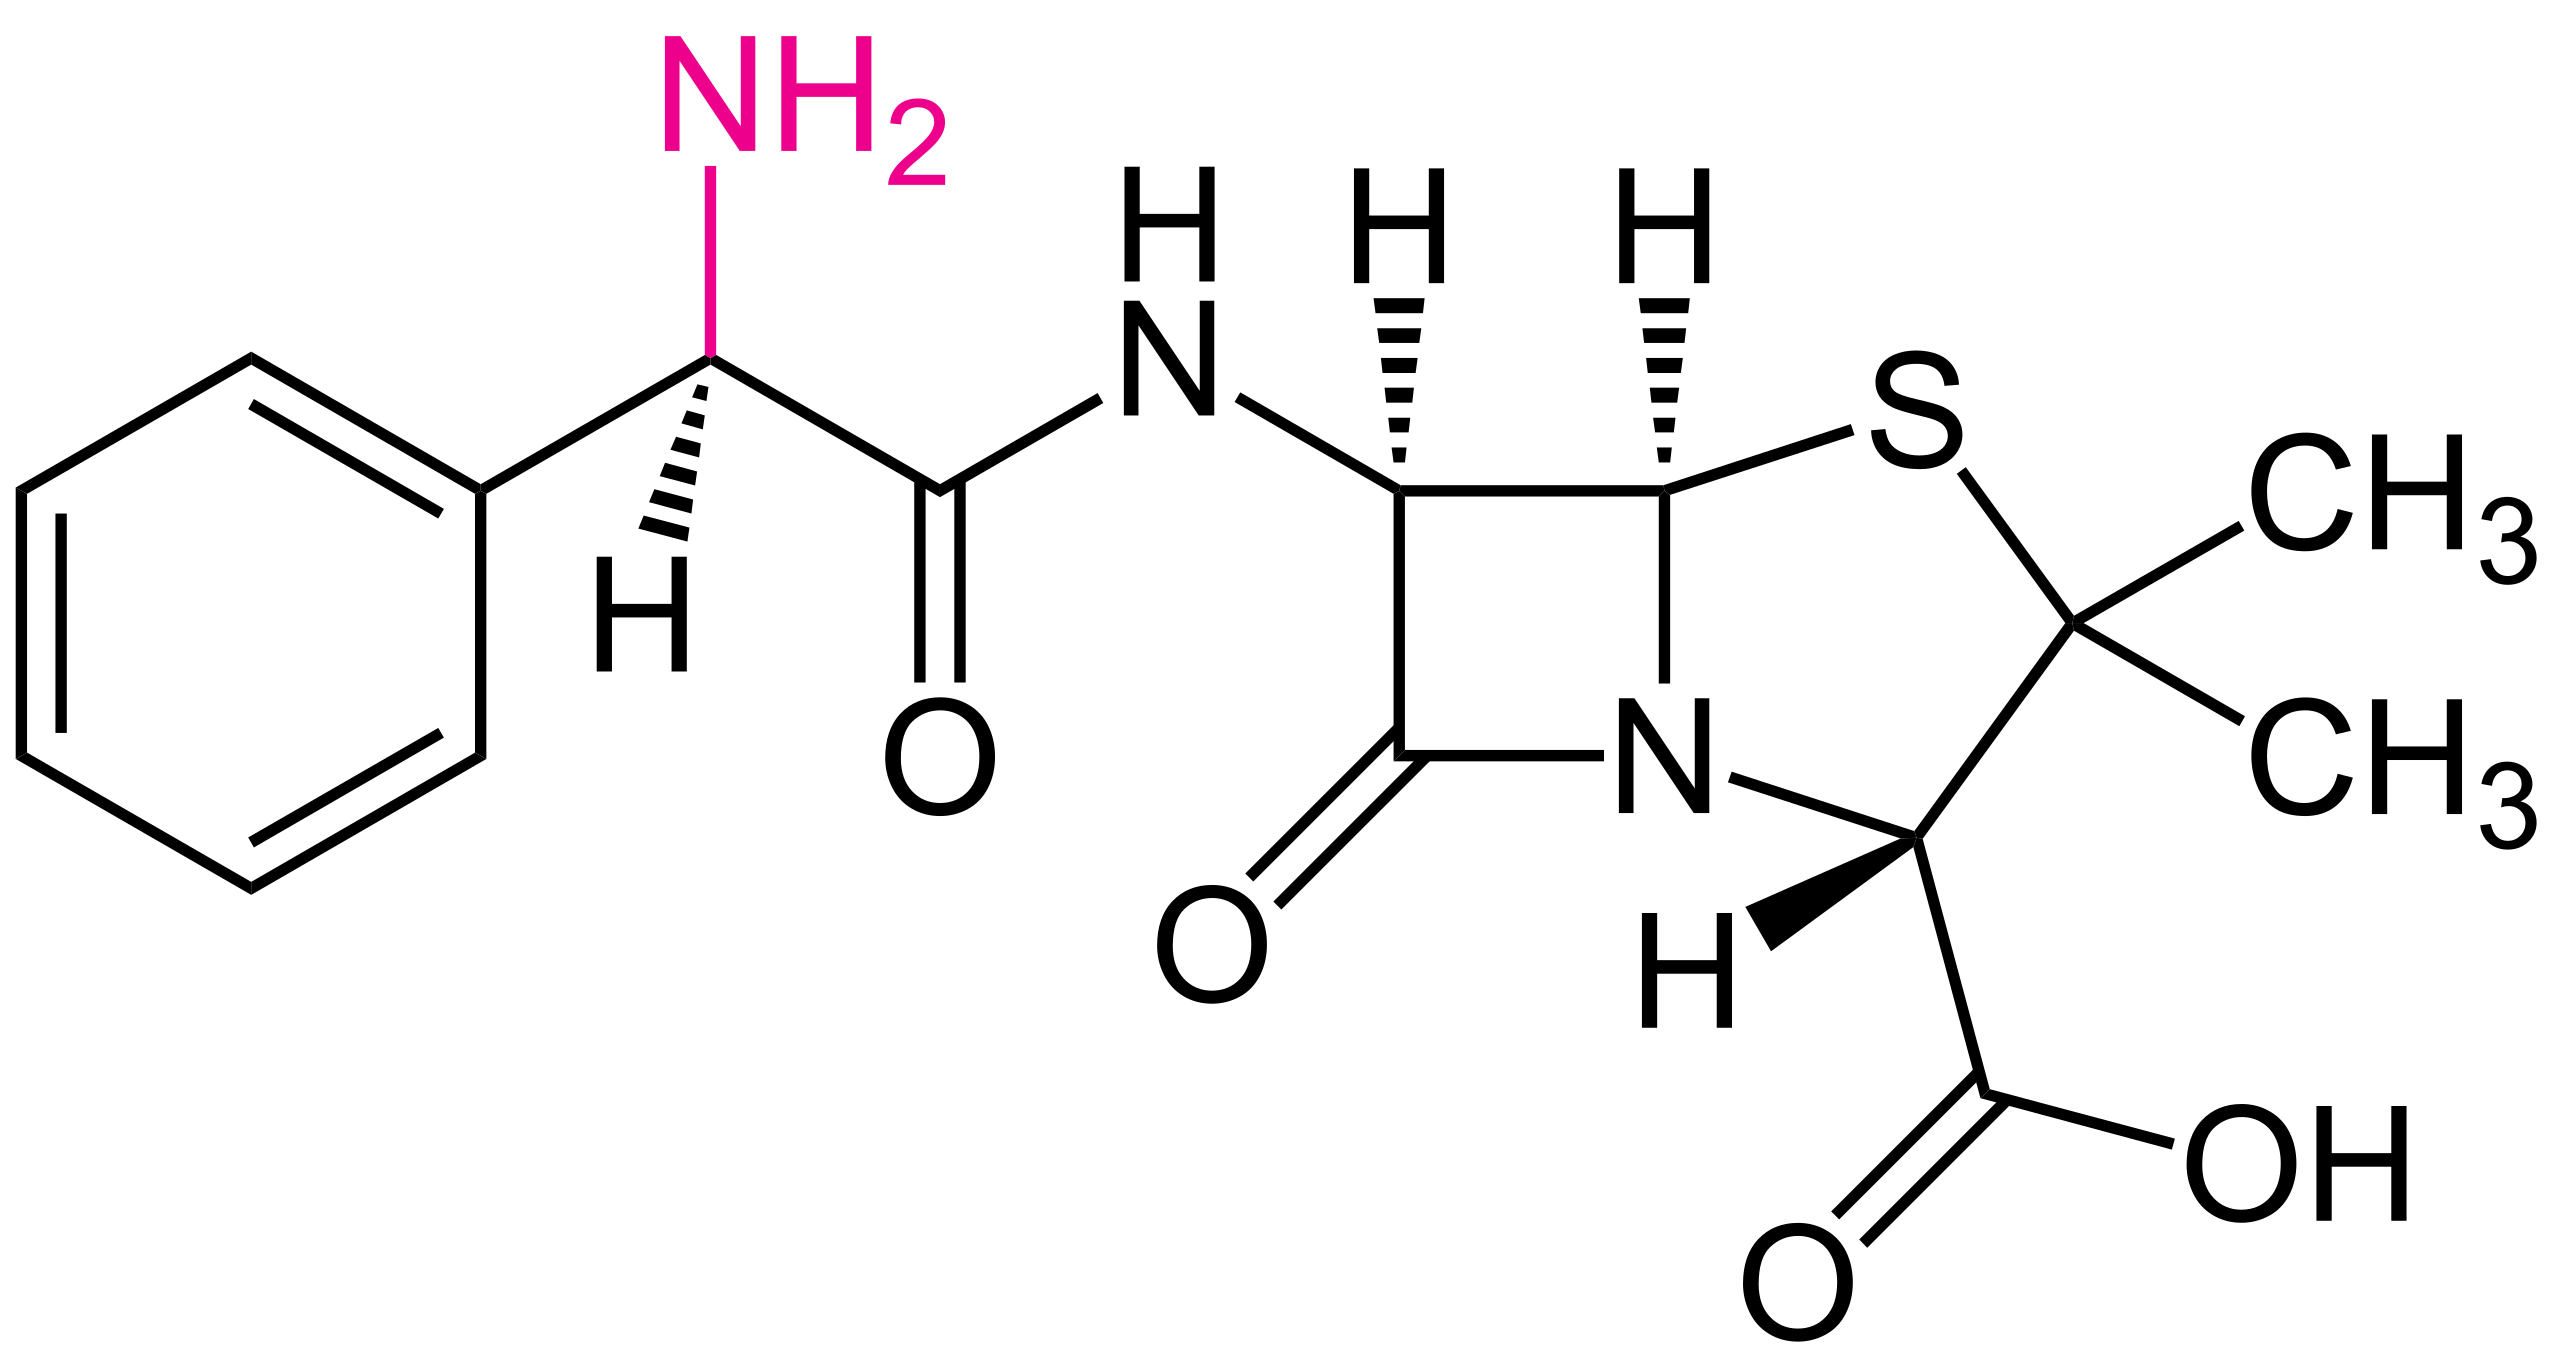
\includegraphics[scale=0.05]{Ampicillin_with_amine_highlighted.png}
            \caption{氨苄青霉素与青霉素G相比在与苯环相连的$\alpha$碳上引入了氨基,使其耐酸并更容易进入细菌细胞膜。}
            \label{fig:label}
        \end{center}
    \end{wrapfigure}
    \indent 氨苄青霉素是青霉素G侧链羧基的$\alpha$位引入氨基,改变了它的极性,使其更容易透过细菌细胞膜。同时它具有耐酸的特征,避免了天然青霉素不宜内服的缺点,为临床给药提供了很大的方便,在临床上得以广泛应用。
    


    % \begin{figure}[ht]
    %     \centering
    %     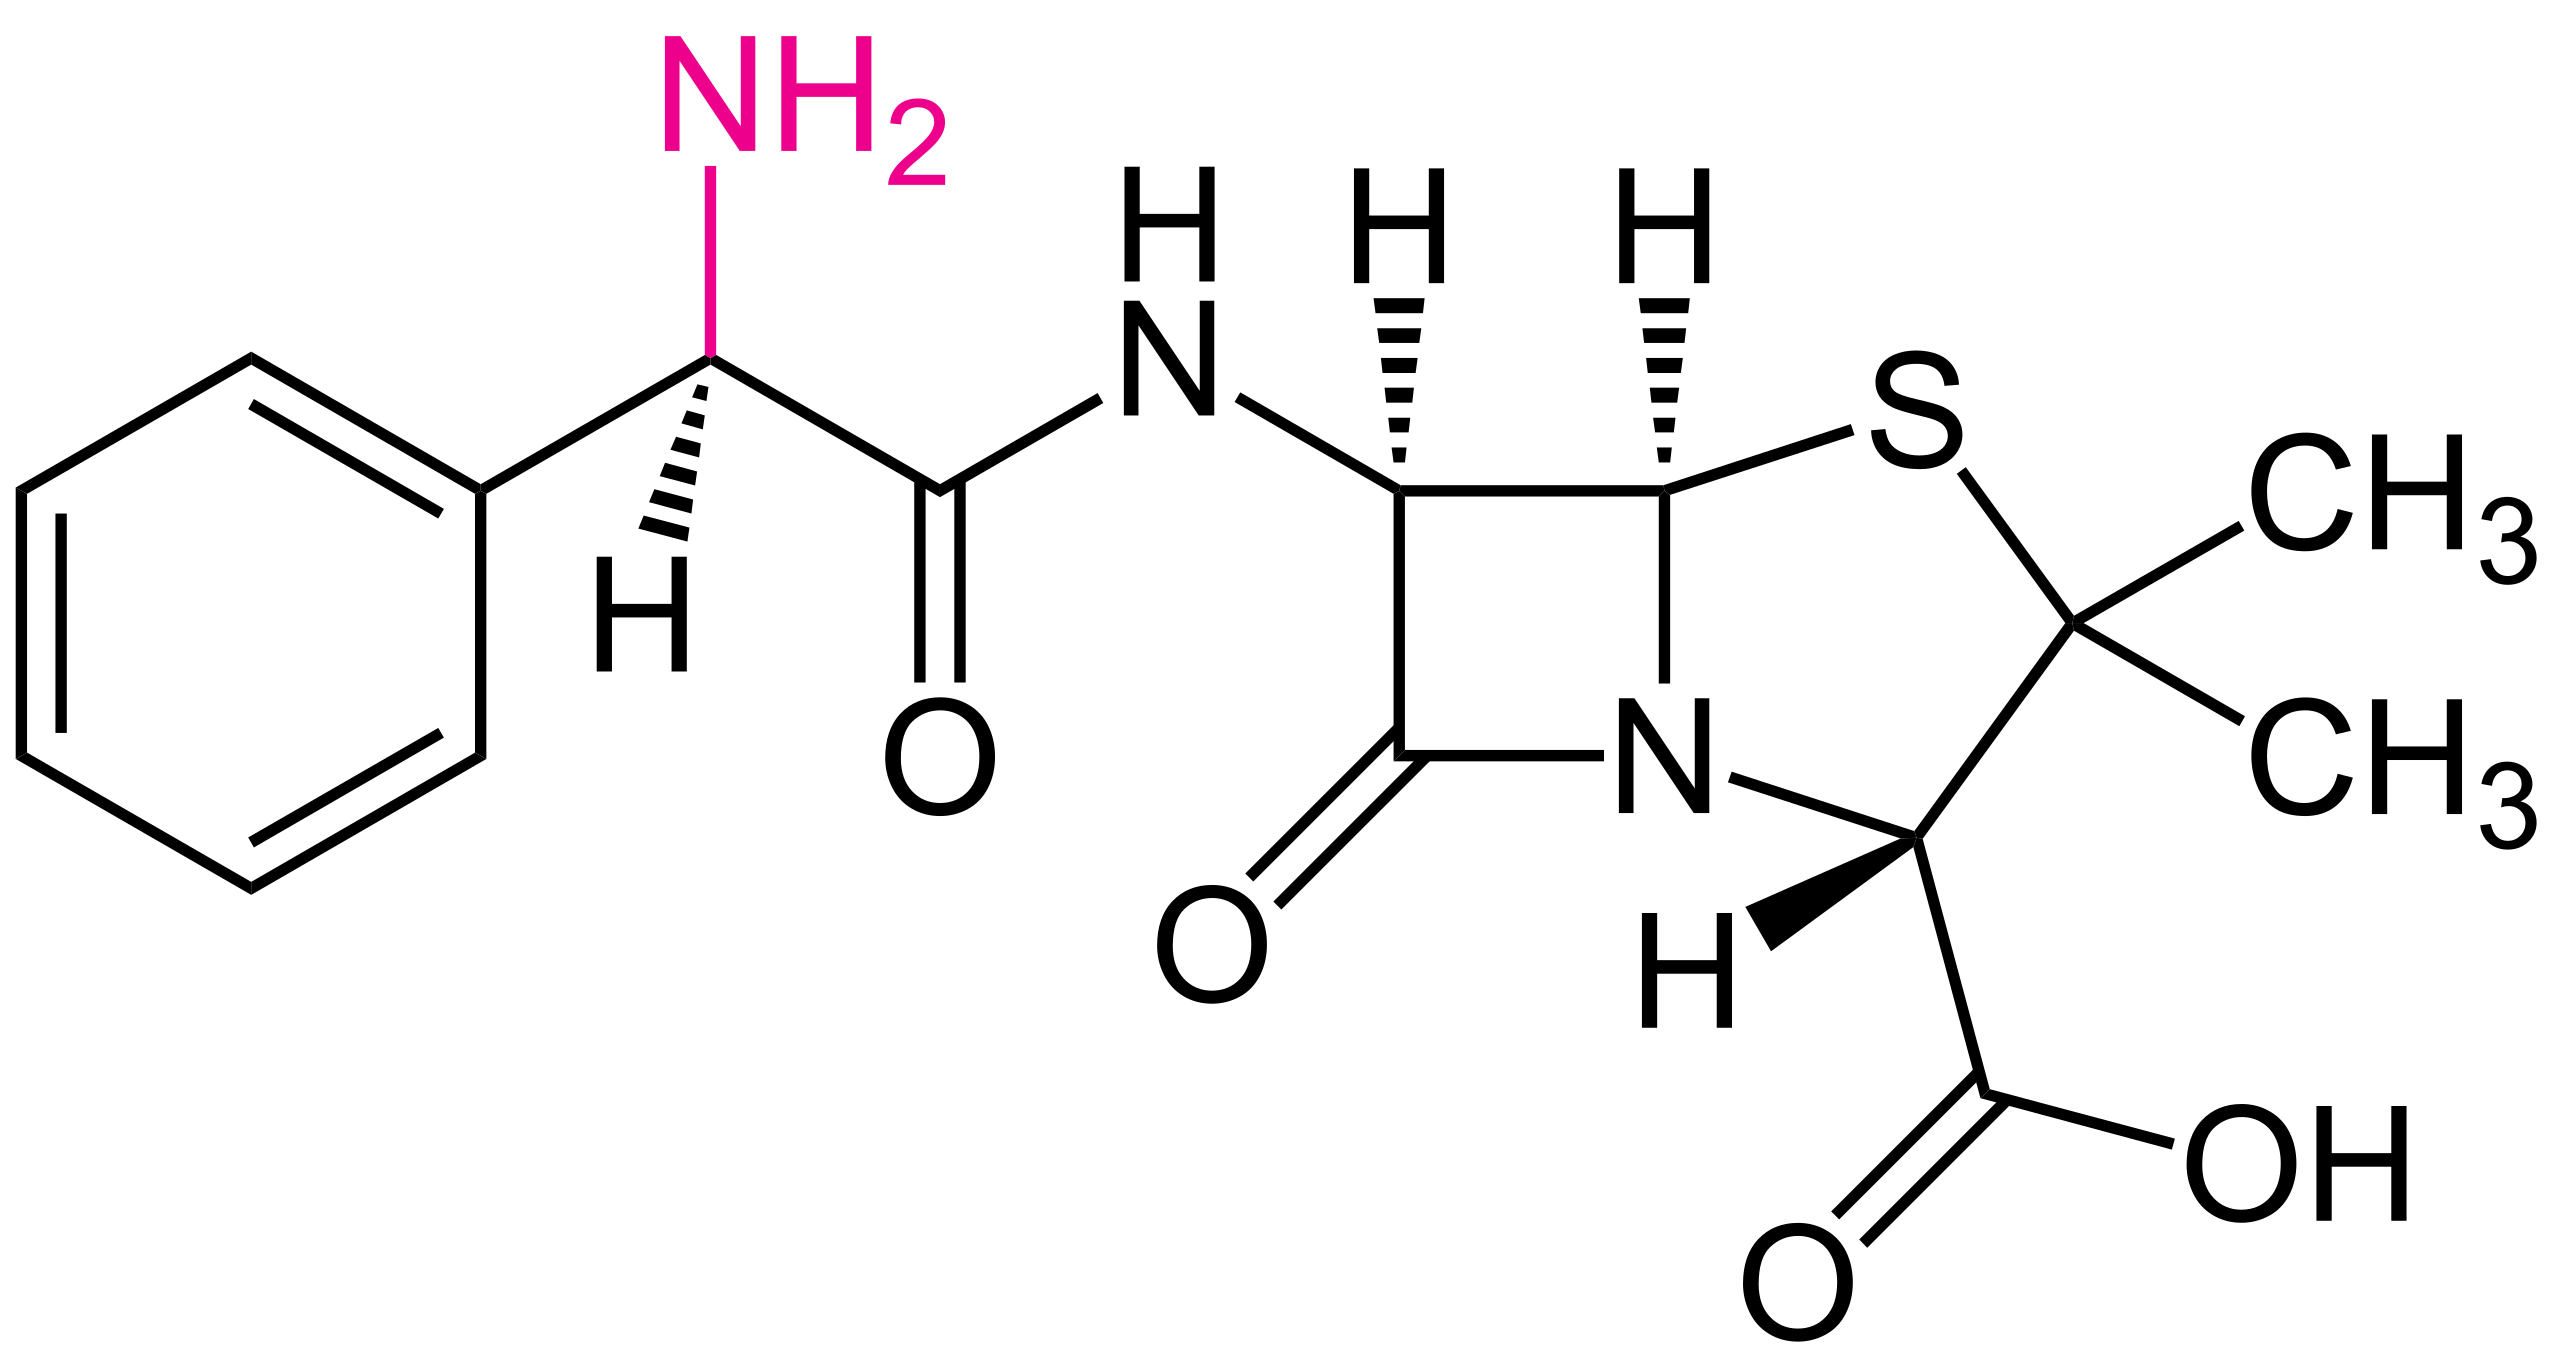
\includegraphics[scale=0.05]{Ampicillin_with_amine_highlighted.png}
    %     \caption{氨苄青霉素与青霉素G相比在与苯环相连的$\alpha$碳上引入了氨基,使其耐酸并更容易进入细菌细胞膜。}
    %     \label{fig:label}
    % \end{figure}
    
    
    
    \section{实验器材}
    \setParDis
    \subsection{菌种}大肠杆菌菌悬液
    \subsection{培养基}LB 固体培养基(三角瓶装)
    \subsection{试剂}生理盐水、氨苄青霉素溶液
    \subsection{器具}
    
    \
    \\
    \indent 无菌Ep管、无菌滤纸圆片(直径5mm)、无菌培养皿、无菌三角形不透明纸板(边长约4cm)、无菌镊子、移液枪及无菌枪头(100\textasciitilde1000μL)、涂布棒、酒精灯、超净工作台、记号笔、封口膜、微波炉、水浴锅、37℃ 培养箱。
    \setParDef

    \section{实验步骤}

    \subsection{研究紫外线对细菌的杀(抑)菌能力(涂布平板法)}
    \begin{enumerate}
        \setlength{\parsep}{-40pt}
        \setlength{\itemsep}{-2pt}
        \item 制平板:取无菌培养皿(直径9cm)6个,将已熔化并冷却至60℃左右的LB固体培养基(三角瓶装)按无菌操作法倒入培养皿中,使冷凝成平板。
        \item 标记和接种:在平板底部标记组别、日期、班级及紫外线照射时间(0s、10s、20s、30s、40s、50s)。用移液枪吸取大肠杆菌菌悬液200ul散落滴加至培养基表面,用涂布棒将菌液在培养基表面均匀涂开。
        \item 紫外线处理:将紫外灯光开灯预热3min。再将上述培养皿置于紫外灯下,将平板按照时间顺序在紫外灯下方摆成一排,并用无菌三角形不透明板遮住细菌涂布面的部分。
        \item 培养:每隔10s取出一块平皿,用封口膜封好,放入37℃恒温培养箱中培养24h。
    \end{enumerate}

    \subsection{研究氨苄青霉素对细菌的杀(抑)菌能力(混合平板法)}
    \begin{enumerate}
        \setlength{\parsep}{-40pt}
        \setlength{\itemsep}{-2pt}
        \item 制平板:取无菌培养皿(直径9cm)1个,用移液枪吸取大肠杆菌菌悬液200μL散落滴加至培养皿中,将已熔化并冷却至60℃左右的LB固体培养基(三角瓶装)按无菌操作法倒入培养皿中,混合均匀,使冷凝成平板。
        \item 标记和接种:在平板底部标记组别、日期、班级,并将培养皿均匀划分为6个区域。用上述同样的方法接种大肠杆菌至培养皿中。
        \item 梯度浓度Amp制备:
            \linespread{1.25}
            \begin{table}[h]
                \centering
                \caption{氨苄青霉素液浓度}
                \begin{tabular}{ccccccc}
                \hline
                管号 & 氨苄青霉素液       & 无菌水          & 10x稀释度       & 100x稀释度      & 1000x稀释度     & 稀释倍数 \\ \hline
                1  & 1000($\mu$L) & -            & -           & -           & -           & 原液   \\
                -  & 100($\mu$L)  & 900($\mu$L)  & -           & -           & -           & 10    \\
                -  & -            & 900($\mu$L)  & 100($\mu$L) & -           & -           & 100   \\
                2  & -            & 900($\mu$L)  & -           & 100($\mu$L) & -           & 1000  \\
                3  & -            & 800($\mu$L)  & -           & 200($\mu$L) & -           & 2000  \\
                4  & -            & 700($\mu$L)  & -           & 300($\mu$L) & -           & 3000  \\
                5  & -            & 600($\mu$L)  & -           & 400($\mu$L) & -           & 4000  \\
                6  & -            & 1000($\mu$L) & -           & -           & -           & 无菌水  \\ \hline
                \end{tabular}
            \end{table}
        \item 按照无菌操作用无菌镊子将六片无菌滤纸圆片(直径0.5cm)分别放入1、2、3、4、5、6号EP管中蘸取氨苄青霉素溶液。
        \item 将蘸取了不同浓度氨苄青霉素溶液的无菌滤纸圆片轻轻平展放置于大肠杆菌培养皿的对应浓度区域中央。
        \item 用封口膜将培养皿封好,放入37℃恒温培养箱中培养24h。

    \end{enumerate}

    \section{实验结果}
    \subsection{紫外线的杀(抑)菌能力}
    \
    \\
    \begin{table}[h]
        \centering
        \caption{紫外线杀菌结果}
        \begin{tabular}{clllllllllll}
        \hline
        培养皿                  & \multicolumn{1}{c}{\quad 0s \qquad} & \multicolumn{2}{c}{10s} & \multicolumn{2}{c}{20s} & \multicolumn{2}{c}{30s} & \multicolumn{2}{c}{40s} & \multicolumn{2}{c}{50s} \\ \hline
        \multicolumn{1}{l}{} &                                                                  & 遮光         & 曝光         & 遮光         & 曝光         & 遮光         & 曝光         & 遮光         & 曝光         & 遮光         & 曝光         \\ \cline{3-12} 
        生长状况                 &                                                                  & \multicolumn{2}{l}{}    & \multicolumn{2}{l}{}    & \multicolumn{2}{l}{}    & \multicolumn{2}{l}{}    & \multicolumn{2}{l}{}    \\ \hline
        \end{tabular}
    \end{table}

    \subsection{氨苄青霉素的杀(抑)菌能力}
    \
    \\
    \begin{table}[h]
        \centering
        \caption{氨苄青霉素杀菌结果}
        \begin{tabular}{lllllll}
        \hline
        培养皿\  & \multicolumn{1}{c}{1} & \multicolumn{1}{c}{2} & \multicolumn{1}{c}{3} & \multicolumn{1}{c}{4} & \multicolumn{1}{c}{5} & \multicolumn{1}{c}{6} \\ \hline
        生长状况 & \qquad\qquad\qquad & \qquad\qquad\qquad & \qquad\qquad\qquad & \qquad\qquad\qquad & \qquad\qquad\qquad & \qquad\qquad\qquad \\ \hline
        \end{tabular}
        \end{table}
    \footnote{*本文采用latex编写,latex源码可见https://github.com/inspirewind/bioinfo-course}

\end{document}